\documentclass[12pt]{memoir}

\def\nsemestre {I}
\def\nterm {Summer}
\def\nyear {2026}
\def\nprofesor {Rosa Orellana}
\def\nauthor {Ignacio Rojas}
\def\nsigla {ECCO}
\def\nsiglahead {Intro to Symmetric Functions}
\def\nlang {ENG}
\let\footruleskip\relax %%FADIR
\input{headerVarillyDiff}
\usepackage{ytableau}

\begin{document}

\chapter{Intro to Symmetric Functions and the Monomial Basis}

% --- Source PDF page 1 ---
\begin{center}
    {\Huge \textbf{Intro to Symmetric Functions and the monomial basis}}\\[1.5em]
    {\Large \textcolor{red}{Rosa Orellana}}\\[0.5em]
    {\large \textcolor{verdeUCR}{Dartmouth College}}\\[0.5em]
    {\large \textbf{CIMPA-ECCO Summer School}}\\[0.5em]
    {\large August 3, 2026}
\end{center}

\newpage

% --- Source PDF page 2 ---
\section{Why symmetric Functions?}

\begin{itemize}[label=$\diamond$]
    \item They encode polynomial Invariance: they are the functions that occur when the variables are unordered.
    \item They describe the roots of polynomials: impossibility of radical formulas.
    \item They provide a powerful enumeration tool.
    \item They describe representations of the symmetric and general linear groups.
    \item They connect to geometry: Schur functions represent Schubert classes in the cohomology of Grassmannians.
    \item They encode graphs: the chromatic symmetric function.
    \item They create a bridge between different disciplines: geometry, physics, probability, topology, graph theory, etc.
    \item They have applications to machine learning: in many data sets the order of the inputs does not matter.
\end{itemize}

\newpage

% --- Source PDF page 3 ---
\section{What is a symmetric polynomial?}

\textbf{Question:} What does a polynomial in variables $x, y$ and $z$ look like if we do not want it to change when we permute the variables?
\[
f(x,y,z) = x^2 + y^2 + z^2
\]

Does this polynomial change when we interchange $x$ and $y$? What about $x$ and $z$?

\textbf{Example:} $g(x,y,z) = x^2 y + x^2 z + y^2 x + y^2 z + z^2 x + z^2 y$ is ``symmetric''.\\
\textbf{Question:} Can you give a concise description of this polynomial without writing all of the terms?

\textbf{Example:} $h(x,y,z) = x^2 y + x^2 z + y^2 x + y^2 z + z^2 x + z^2 y + 2x^3 + 2y^3 + 2z^3$ is also ``symmetric''.

\begin{itemize}[label=$\diamond$]
    \item We have seen that our polynomials will have several \textcolor{red}{variables}, we will use for any positive integer $n$
    \[
    x_1, x_2, x_3, \dots, x_n
    \]
    For our variables.
    \item The \textcolor{red}{coefficients} of the polynomials will come from $\mathbb{Q}$ (rational numbers, fractions).
    \[
    g(x,y,z) = x_1^2 x_2 + x_1^2 x_3 + x_2^2 x_1 + x_2^2 x_3 + x_3^2 x_1 + x_3^2 x_2
    \]
    \item We need an \textcolor{red}{``action''} of the \textcolor{red}{symmetric group} to formalize the ``interchange'' of the variables.
\end{itemize}

\newpage

% --- Source PDF page 4 ---
\section{Symmetric group and action on polynomials}

\begin{itemize}[label=$\diamond$]
    \item The \textcolor{red}{symmetric group $S_n$} is the group of all bijections from $[n] := \{1,2,\dots,n\}$ to itself.
\end{itemize}

\textbf{Example:} When $n = 3$
\[
S_3 = \left\{ 
\begin{pmatrix} 1 & 2 & 3 \\ 1 & 2 & 3 \end{pmatrix}, 
\begin{pmatrix} 1 & 2 & 3 \\ 1 & 3 & 2 \end{pmatrix}, 
\begin{pmatrix} 1 & 2 & 3 \\ 2 & 1 & 3 \end{pmatrix}, 
\begin{pmatrix} 1 & 2 & 3 \\ 2 & 3 & 1 \end{pmatrix}, 
\begin{pmatrix} 1 & 2 & 3 \\ 3 & 1 & 2 \end{pmatrix}, 
\begin{pmatrix} 1 & 2 & 3 \\ 3 & 2 & 1 \end{pmatrix} 
\right\}
\]

\begin{itemize}[label=$\diamond$]
    \item The action of $S_n$ on a polynomial with $n$ variables, is defined for $\pi \in S_n$,
    \[
    \pi \cdot f(x_1, x_2, \dots, x_n) = f(x_{\pi(1)}, x_{\pi(2)}, \dots, x_{\pi(n)})
    \]
\end{itemize}

\textbf{Example:} $\pi = \begin{pmatrix} 1 & 2 & 3 \\ 3 & 1 & 2 \end{pmatrix}$ and $f(x_1, x_2, x_3) = x_1^2 x_2^2 x_3 + x_1^2 x_3^2 x_2 + x_2^2 x_3^2 x_1$\\
Then
\[
\begin{aligned}
\pi \cdot f(x_1, x_2, x_3) &= x_{\pi(1)}^2 x_{\pi(2)}^2 x_{\pi(3)} + x_{\pi(1)}^2 x_{\pi(3)}^2 x_{\pi(2)} + x_{\pi(2)}^2 x_{\pi(3)}^2 x_{\pi(1)}\\ 
&= x_3^2 x_1^2 x_2 + x_3^2 x_2^2 x_1 + x_1^2 x_2^2 x_3
\end{aligned}
\]
\textbf{NOTE:} $\pi \cdot f(x_1, x_2, x_3) = f(x_1, x_2, x_3)$

\textbf{Example:} $\pi = \begin{pmatrix} 1 & 2 & 3 & 4 \\ 2 & 4 & 1 & 3 \end{pmatrix}$ and $f(x_1, x_2, x_3, x_4) = x_1^2 + 3x_2 x_4 - 2x_3^2 x_4$\\
Then
\[
\pi \cdot f(x_1, x_2, x_3, x_4) = x_{\pi(1)}^2 + 3x_{\pi(2)} x_{\pi(4)} - 2x_{\pi(3)}^2 x_{\pi(4)} = x_2^2 + 3x_4 x_3 - 2x_1^2 x_3
\]
\textbf{NOTE:} $\pi \cdot f(x_1, x_2, x_3, x_4) \neq f(x_1, x_2, x_3, x_4)$

\begin{ptcb}
\begin{Prop}[\textbf{Properties of the action}]
Let $c \in \mathbb{Q}$, $f$ and $g$ polynomials and $\sigma, \pi \in S_n$. Then
\begin{enumerate}[(i)]
    \item $\pi \cdot (cf) = c(\pi \cdot f)$
    \item $\pi \cdot (f + g) = \pi \cdot f + \pi \cdot g$
    \item $\pi \cdot (fg) = (\pi \cdot f)(\pi \cdot g)$
    \item $(\pi \sigma) \cdot f = \pi \cdot (\sigma \cdot f)$
\end{enumerate}
\end{Prop}
\end{ptcb}

\newpage

% --- Source PDF page 5 ---
\section{Definition of symmetric polynomial}

\begin{ptcb}
\begin{Def}
A polynomial $f(x_1, x_2, \dots, x_n)$ is called \textcolor{red}{symmetric} if $\pi \cdot f(x_1, \dots, x_n) = f(x_1, \dots, x_n)$ for all $\pi \in S_n$.
\end{Def}
\end{ptcb}

We use $\Lambda(x_1, \dots, x_n)$ or $\Lambda_n$ for the set of all symmetric polynomials in $n$ variables.

\textbf{Example:} $x_1^2 x_2 + x_1^2 x_3 + x_2^2 x_1 + x_2^2 x_3 + x_3^2 x_1 + x_3^2 x_2 \in \Lambda_3$.

\begin{itemize}[label=$\diamond$]
    \item Since we can add and scale symmetric polynomials and get a symmetric polynomial, $\Lambda_n$ is an infinite dimensional vector space.
\end{itemize}

\begin{ptcb}
\begin{Def}
A polynomial $f(x_1, x_2, \dots, x_n)$ is \textcolor{red}{homogeneous of degree $k$} if every one of its monomials has degree $k$.
\end{Def}
\end{ptcb}

\begin{itemize}[label=$\diamond$]
    \item We use $\Lambda_n^k$ for the set of all homogenous symmetric polynomials of degree $k$.
    \item \textbf{Note:} Every monomial in the $0$ polynomial has degree $k$ (since it has no monomials), so $0 \in \Lambda_n^k$.
    \item $\Lambda_n$ can be decomposed into its homogeneous pieces:
    \[
    \Lambda_n = \Lambda_n^0 \oplus \Lambda_n^1 \oplus \Lambda_n^2 \oplus \dots = \bigoplus_k \Lambda_n^k \qquad \text{\textbf{Note: }} \Lambda_n^0 = \mathbb{Q}.
    \]
    \item What does this say? If $f \in \Lambda_n$, then $f = f_0 + f_1 + f_2 + \dots$, where $f_i \in \Lambda_n^i$.
    \item $\Lambda_n^k$ is finite dimensional, and we concentrate on understanding these homogeneous spaces.
\end{itemize}

\newpage

% --- Source PDF page 6 ---
\section{Understanding \texorpdfstring{$\Lambda_n^k$}{Lambda\_n\^{}k}}

The first step to understand a vector space is to find a linear basis for it.

\textbf{Question:} What is the symmetric polynomial with the smallest number of monomials that contains $x_1^2 x_2$ in $\Lambda_3^3$ ?

\textbf{Question:} What is the symmetric polynomial with the smallest number of monomials that contains $x_1^3$ in $\Lambda_3^3$ ?

\textbf{Question:} What is the symmetric polynomial with the smallest number of monomials that contains $x_1 x_2 x_3$ in $\Lambda_3^3$ ?

\textbf{Question:} How can we describe these polynomials without listing all the monomials?

\textcolor{red}{\textbf{Algebra Note:}} We can think of the symmetric group $S_n$ acting on the set of all monomials:\\
For $n = 3$ and $k = 3$ the set is $\{x_1 x_2 x_3, x_1^2 x_2, x_1^2 x_3, x_2^2 x_1, x_2^2 x_3, x_3^2 x_1, x_3^2 x_2, x_1^3, x_2^3, x_3^3\}$

\textbf{Question:} What are the orbits of the action?
\begin{align*}
    O_1 &= \{x_1 x_2 x_3\}\\
    O_2 &= \{x_1^2 x_2, x_1^2 x_3, x_2^2 x_1, x_2^2 x_3, x_3^2 x_1, x_3^2 x_2\}\\
    O_3 &= \{x_1^3, x_2^3, x_3^3\}
\end{align*}

\textbf{Question:} How can we ``index'' these orbits, what is their defining property? \textcolor{blue}{\textbf{PARTITIONS!}}

\textbf{Note:} the polynomials we got above are the sum of the elements in the orbits. The partitions of $k = 3$ are $(1,1,1)$, $(2,1)$ and $(3)$
\begin{align*}
    m_{1,1,1} &= x_1 x_2 x_3\\
    m_{2,1} &= x_1^2 x_2 + x_1^2 x_3 + x_2^2 x_1 + x_2^2 x_3 + x_3^2 x_1 + x_3^2 x_2\\
    m_3 &= x_1^3 + x_2^3 + x_3^3
\end{align*}

\newpage

% --- Source PDF page 7 ---
\section{Partitions}

\begin{ptcb}
\begin{Def}
For any nonnegative integer $k$, a \textcolor{red}{partition $\lambda$} of $k$ is a weakly decreasing sequence of nonnegative integers $\lambda = (\lambda_1, \lambda_2, \dots, \lambda_\ell)$ such that $\lambda_1 + \lambda_2 + \dots + \lambda_\ell = k$.
\end{Def}
\end{ptcb}

\textbf{Example:} The partitions of $k = 5$ are $(5), (4,1), (3,2), (3,1,1), (2,2,1), (2,1,1,1)$, and $(1,1,1,1,1)$

If $\lambda$ is a partition of $k$, we write $\lambda \vdash k$ or $|\lambda| = \lambda_1 + \lambda_2 + \dots + \lambda_\ell = k$.

The $\lambda_i$ are called \textcolor{red}{parts}, and the number of nonzero parts is called the \textcolor{red}{length} of $\lambda$ and we write $\ell(\lambda)$.

We use exponent notation for partitions: $(k^{m_k}, (k-1)^{m_{k-1}}, \dots, 2^{m_2}, 1^{m_1})$

For example, $(5,5,5,4,3,3,3,3,3,1,1,1,1) = (5^3, 4^1, 3^5, 1^4)$.

We call the $m_i$ \textcolor{red}{multiplicities}, and this means there are $m_i$ parts $i$ in $\lambda$.\\
For example in the partition above, $5$ has multiplicity $3$, so $m_5 = 3$.

The \textcolor{red}{\textbf{Young diagram:}} It is useful to associate a geometric picture to a partition.

For example, $(5,3,3,2,1)$ has Young diagram:
\begin{center}
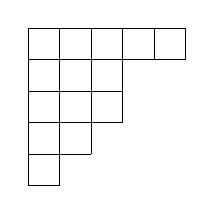
\begin{tikzpicture}[scale=0.4]
    \draw (0,0) grid (5,-1);
    \draw (0,-1) grid (3,-3);
    \draw (0,-3) grid (2,-4);
    \draw (0,-4) grid (1,-5);
\end{tikzpicture}
\end{center}

\newpage

% --- Source PDF page 8 ---
\section{Partitions (continued)}

\begin{itemize}[label=$\diamond$]
    \item The \textcolor{red}{conjugate} of a partition $\lambda$ is the partition $\lambda'$ with parts the column lengths of the Young diagram of $\lambda$.
\end{itemize}

\begin{center}
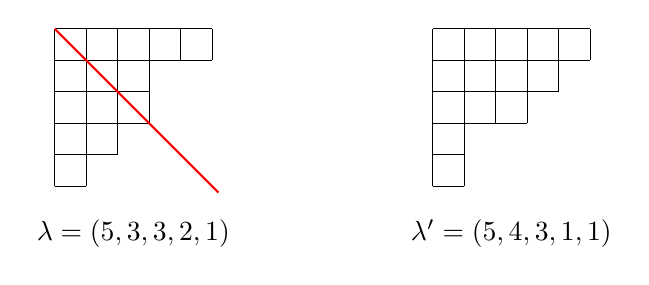
\begin{tikzpicture}[scale=0.4]
    % Left diagram
    \begin{scope}[shift={(0,0)}]
        \draw (0,0) grid (5,-1);
        \draw (0,-1) grid (3,-3);
        \draw (0,-3) grid (2,-4);
        \draw (0,-4) grid (1,-5);
        \draw[red, thick] (0,0) -- (5.2,-5.2);
        \node at (2.5,-6.5) {$\lambda = (5,3,3,2,1)$};
    \end{scope}
    
    % Right diagram
    \begin{scope}[shift={(12,0)}]
        \draw (0,0) grid (5,-1);
        \draw (0,-1) grid (4,-2);
        \draw (0,-2) grid (3,-3);
        \draw (0,-3) grid (1,-5);
        \node at (2.5,-6.5) {$\lambda' = (5,4,3,1,1)$};
    \end{scope}
\end{tikzpicture}
\end{center}

\begin{itemize}[label=$\diamond$]
    \item The conjugate map is an involution, $(\lambda')' = \lambda$. It is a bijection!
    \item The number of partitions will be the number $p(k)$.
\end{itemize}

\begin{center}
\begin{tabular}{c|ccccccccc}
$k$ & 0 & 1 & 2 & 3 & 4 & 5 & 6 & 7 & 8 \\
\hline
$p(k)$ & 1 & 1 & 2 & 3 & 5 & 7 & 11 & 15 & 22
\end{tabular}
\end{center}

\begin{itemize}[label=$\diamond$]
    \item The generating function for partitions:
\end{itemize}

\begin{ptcb}
\textbf{Euler's Theorem:} 
\[
\sum_{k=0}^\infty p(k) x^k = \prod_{i=1}^\infty \frac{1}{1 - x^i}
\]
\end{ptcb}

\newpage

% --- Source PDF page 9 ---
\section{The monomial symmetric polynomials}

\begin{ptcb}
\begin{Def}
For $n \ge 1$ and a partition $\lambda$, the \textcolor{red}{monomial symmetric polynomial $m_\lambda(x_1, \dots, x_n)$} indexed by $\lambda$ is the sum of the monomial $x_1^{\lambda_1} x_2^{\lambda_2} \dots x_{\ell(\lambda)}^{\lambda_{\ell(\lambda)}}$ and all the possible \textcolor{blue}{different} monomials $\pi \cdot (x_1^{\lambda_1} x_2^{\lambda_2} \dots x_{\ell(\lambda)}^{\lambda_{\ell(\lambda)}})$ obtained by acting by $\pi \in S_n$.

\textbf{Note:} If $\ell(\lambda) > n$, then $m_\lambda(x_1, \dots, x_n) = 0$ because we assume that $x_j = 0$ for $j > n$.
\end{Def}
\end{ptcb}

\textcolor{verdeUCR}{\textbf{Examples:}}
\begin{align*}
    m_{2,1}(x_1, x_2) &= x_1^2 x_2 + x_1 x_2^2\\[0.5em]
    m_{2,1}(x_1, x_2, x_3) &= x_1^2 x_2 + x_1 x_2^2 + x_1^2 x_3 + x_2^2 x_3 + x_1 x_3^2 + x_2 x_3^2\\[0.5em]
    m_{3,3,1,1}(x_1, x_2, x_3, x_4) &= x_1^3 x_2^3 x_3 x_4 + x_1^3 x_2 x_3^3 x_4 + x_1^3 x_2 x_3 x_4^3\\
    &\quad + x_1 x_2^3 x_3^3 x_4 + x_1 x_2^3 x_3 x_4^3 + x_1 x_2 x_3^3 x_4^3\\[0.5em]
    m_k(x_1, x_2, x_3, x_4) &= x_1^k + x_2^k + x_3^k + x_4^k\\[0.5em]
    m_{1,1,1}(x_1, x_2, x_3, x_4) &= x_1 x_2 x_3 + x_1 x_2 x_4 + x_1 x_3 x_4 + x_2 x_3 x_4
\end{align*}

\newpage

% --- Source PDF page 10 ---
\section{The monomial symmetric functions are symmetric}

\begin{ptcb}
\begin{Prop}
For all positive integers $n$ and all partitions $\lambda$, the polynomial $m_\lambda(x_1, \dots, x_n)$ is a symmetric polynomial in $x_1, x_2, \dots, x_n$.
\end{Prop}
\end{ptcb}

\begin{proof}
If $n < \ell(\lambda)$, then $m_\lambda(x_1, \dots, x_n) = 0$, which is symmetric.\\
Otherwise, let $\sigma_i = (i, i+1)$ be the permutation in $S_n$ that maps $i$ to $i+1$ and $i+1$ to $i$ and maps all other $j \neq i, i+1$ to $j$ ($j \to j$).\\
\textbf{Claim:} $\sigma_i \cdot m_\lambda(x_1, \dots, x_n) = m_\lambda(x_1, \dots, x_n)$ for any $1 \le i \le n-1$.\\
To show this we must show that every monomial $x_1^{\alpha_1} x_2^{\alpha_2} \dots x_n^{\alpha_n}$ in $\sigma_i \cdot m_\lambda(x_1, \dots, x_n)$ has the same coefficient in both $\sigma_i \cdot m_\lambda(x_1, \dots, x_n)$ and $m_\lambda(x_1, \dots, x_n)$.\\
Note that the coefficient of $x_1^{\alpha_1} x_2^{\alpha_2} \dots x_n^{\alpha_n}$ is $1$ in $m_\lambda(x_1, \dots, x_n)$ if $(\alpha_1, \alpha_2, \dots, \alpha_n)$ is a reordering of $\lambda$ (we could add some zeros at the end of $\lambda$ as some $\alpha_j$'s could be zero) and the coefficient is zero otherwise.

On the other hand, the coefficient of $x_1^{\alpha_1} \dots x_i^{\alpha_{i+1}} x_{i+1}^{\alpha_i} \dots x_n^{\alpha_n}$ in $\sigma_i \cdot m_\lambda(x_1, \dots, x_n)$ is the same as the coefficient of $x_1^{\alpha_1} \dots x_i^{\alpha_i} x_{i+1}^{\alpha_{i+1}} \dots x_n^{\alpha_n}$ in $m_\lambda(x_1, \dots, x_n)$ since permutation does not change the coefficients. And the coefficient is $1$ if $(\alpha_1, \alpha_2, \dots, \alpha_n)$ is a reordering of $\lambda$ and zero otherwise.

But $(\alpha_1, \alpha_2, \dots, \alpha_n)$ is a reordering of $\lambda$ if and only if $(\alpha_1, \alpha_2, \dots, \alpha_{i+1}, \alpha_i, \dots, \alpha_n)$ is also a reordering of $\lambda$. Therefore, the claim follows.
\end{proof}

\newpage

% --- Source PDF page 11 ---
\section{The monomial symmetric polynomials form a basis for \texorpdfstring{$\Lambda_n^k$}{Lambda\_n\^{}k}}

\begin{ptcb}
\begin{Prop}
If $n \ge 1$, $k \ge 0$, and $n \ge k$, then $\{m_\lambda(x_1, \dots, x_n) \mid \lambda \vdash k\}$ is a basis for $\Lambda_n^k$. In particular, $\dim(\Lambda_n^k) = p(k)$, the number of partitions of $k$.
\end{Prop}
\end{ptcb}

\begin{proof}
Note that if $\lambda \neq \mu$, then $m_\lambda(x_1, \dots, x_n)$ and $m_\mu(x_1, \dots, x_n)$ have no terms in common.\\
And $m_\lambda(x_1, \dots, x_n) \neq 0$ for all $\lambda \vdash k$ because $n \ge k$. Then
\[
\sum_{\lambda \vdash k} a_\lambda m_\lambda(x_1, \dots, x_n) = 0
\]
if and only if $a_\lambda = 0$ for all $\lambda \vdash k$. Therefore, $\{m_\lambda(x_1, \dots, x_n) \mid \lambda \vdash k\}$ is linearly independent.

Now we show that $\{m_\lambda(x_1, \dots, x_n) \mid \lambda \vdash k\}$ spans $\Lambda_n^k$. Let $f \in \Lambda_n^k$, if $f = 0$, we are done. So assume $f \neq 0$. We use induction on the number of monomials in $f$ to show that $f = \sum_\lambda c_\lambda m_\lambda(x_1, \dots, x_n)$.

Since $f \neq 0$, it has a term $c x_1^{\alpha_1} \dots x_n^{\alpha_n}$ with $c \in \mathbb{Q}$ and not equal to zero and $\alpha \vdash k$. Since $f$ is symmetric, then for every $\pi \in S_n$, $\pi \cdot (c x_1^{\alpha_1} \dots x_n^{\alpha_n}) = c \pi \cdot (x_1^{\alpha_1} \dots x_n^{\alpha_n})$ is also a term in $f$. Therefore, $f - c m_\alpha \in \Lambda_n^k$ and has fewer terms than $f$. By induction $f - c m_\alpha$ is a linear combination of the $m_\lambda(x_1, \dots, x_n)$'s. Thus $\{m_\lambda(x_1, \dots, x_n) \mid \lambda \vdash k\}$ spans $\Lambda_n^k$.

Hence, $\{m_\lambda(x_1, \dots, x_n) \mid \lambda \vdash k\}$ is a basis and therefore the dimension is the $p(k)$.
\end{proof}

\newpage

% --- Source PDF page 12 ---
\section{Symmetric Functions}

\textbf{Note:} If $n \ge k$, then $\dim(\Lambda_n^k) = p(k)$ and it is independent of $n$.\\
If we let $n \to \infty$, the polynomials $m_\lambda(x_1, x_2, \dots, x_n)$ become power series.

\begin{align*}
    m_{2,1}(x_1, x_2) &= x_1^2 x_2 + x_1 x_2^2\\[0.5em]
    m_{2,1}(x_1, x_2, x_3) &= x_1^2 x_2 + x_1 x_2^2 + \textcolor{red}{x_1^2 x_3 + x_2^2 x_3 + x_1 x_3^2 + x_2 x_3^2}\\[0.5em]
    m_{2,1}(x_1, x_2, x_3, x_4) &= x_1^2 x_2 + x_1 x_2^2 + x_1^2 x_3 + x_2^2 x_3 + x_1 x_3^2 + x_2 x_3^2\\
    &\quad + \textcolor{red}{x_1^2 x_4 + x_2^2 x_4 + x_3^2 x_4 + x_1 x_4^2 + x_2 x_4^2 + x_3 x_4^2}
\end{align*}

\[
\textcolor{celesUCR}{m_{2,1} = m_{2,1}(x_1, x_2, \dots) = \sum_{1 \le i \neq j \le \infty} x_i^2 x_j}
\]

A power series is like an infinite polynomial. And it is called a \textcolor{red}{function} if it has bounded degree, that is the sum of the exponents is finite for every monomial.\\
Hence, a \textcolor{red}{symmetric function} is a power series with bounded degree such that it doesn't change when we permute the variables:
\[
\textcolor{celesUCR}{f = \sum c_\alpha x^\alpha \qquad (\text{here } x^\alpha \text{ is short for } x_1^{\alpha_1} x_2^{\alpha_2} \dots)}
\]
$\alpha = (\alpha_1, \alpha_2, \dots)$ is a sequence of nonnegative integer and $\alpha_1 + \alpha_2 + \dots$ is bounded and $\pi \cdot f = f$.

\begin{ptcb}
\begin{Prop}
For any $\lambda$, if $n \ge \ell(\lambda)$, then $m_\lambda(x_1, x_2, \dots, x_n, 0, \dots, 0) = m_\lambda(x_1, \dots, x_n)$.
\end{Prop}
\end{ptcb}

\begin{proof}
We can see that $m_\lambda(x_1, x_2, \dots, x_n, 0) = m_\lambda(x_1, \dots, x_n)$ because they are the sum of the same monomials, and the general result follows by induction.
\end{proof}

\newpage

% --- Source PDF page 13 ---
\section{Multiplying power series}

Given $F(x) = \sum_{i=0}^\infty a_i x^i$ and $G(x) = \sum_{i=0}^\infty b_i x^i$, then $F(x)G(x) = \sum_{k=0}^\infty c_k x^k$ where $c_k = \sum_{i=0}^k a_i b_{k-i}$

Geometric Series: $\sum_{i=0}^\infty x^i = \frac{1}{1 - x}$

\textcolor{verdeUCR}{\textbf{Example:}} What is $\left( \sum_{i=0}^\infty x^i \right)\left( \sum_{i=0}^\infty x^i \right)$ ?

\[
\left( \sum_{i=0}^\infty x^i \right)\left( \sum_{i=0}^\infty x^i \right) = (1 + x + x^2 + x^3 + \dots)(1 + x + x^2 + x^3 + \dots) = 1 + 2x + 3x^2 + 4x^3 + \dots
\]

The coefficient is: $c_k = \sum_{i=0}^k (1)(1) = k + 1$

What about multivariate power series?

\textcolor{verdeUCR}{\textbf{Example:}} What is $m_1 m_1$ ?

\[
m_1 m_1 = (x_1 + x_2 + x_3 + \dots)(x_1 + x_2 + x_3 + \dots)
\]

We get quadratic polynomials: $x_i^2$ and $x_i x_j$ with $i \neq j$ what are their coefficients?\\
To get $x_1^2$ we must pick $x_1$ from both factors, so coefficient is 1. We can get $x_1 x_2$ in two ways pick $x_1$ from either first or second factor (two choices) and the $x_2$ from the other factor.
\[
m_1 m_1 = m_2 + 2m_{1,1}
\]

\newpage

% --- Source PDF page 14 ---
\section{Multiplying monomial symmetric functions}

\begin{center}
\begin{tabular}{c|l}
$n$ & $m_{1,1}(x_1, \dots, x_n) m_{2,1}(x_1, \dots, x_n)$ \\
\hline
2 & $m_{3,2}$ \\
3 & $m_{3,2} + 2m_{3,1,1} + 2m_{2,2,1}$ \\
4 & $m_{3,2} + 2m_{3,1,1} + 2m_{2,2,1} + 3m_{2,1,1,1}$ \\
5 & $m_{3,2} + 2m_{3,1,1} + 2m_{2,2,1} + 3m_{2,1,1,1}$ \\
6 & $m_{3,2} + 2m_{3,1,1} + 2m_{2,2,1} + 3m_{2,1,1,1}$ \\
7 & $m_{3,2} + 2m_{3,1,1} + 2m_{2,2,1} + 3m_{2,1,1,1}$
\end{tabular}
\end{center}

\textbf{Note:} the product stabilizes when you have ``enough'' variables and stays the same.\\
It will be enough to compute the coefficient of $x_1^{\alpha_1} \dots x_{\alpha_\ell}^{\alpha_\ell}$ because the product is symmetric.

\begin{ptcb}
\begin{Prop}
For any partitions $\lambda, \mu$ and $\nu \vdash |\lambda| + |\mu|$, the coefficients $a_{\lambda,\mu}^\nu$ in the product
\[
m_\lambda(x_1, \dots, x_n) m_\mu(x_1, \dots, x_n) = \sum_{\nu \vdash |\lambda| + |\mu|} a_{\lambda,\mu}^\nu m_\nu(x_1, \dots, x_n)
\]
do not depend on $n$ when $n \ge \ell(\lambda) + \ell(\mu)$ and
\[
m_\lambda m_\mu = \sum_{\nu \vdash |\lambda| + |\mu|} a_{\lambda,\mu}^\nu m_\nu
\]
i.e., for the functions the coefficients are the same.
\end{Prop}
\end{ptcb}

\newpage

% --- Source PDF page 15 ---
\section{The monomial symmetric functions form a basis}

We use \textcolor{celesUCR}{$\Lambda$} for the ring of symmetric functions.\\
And \textcolor{celesUCR}{$\Lambda^k$} for the homogeneous symmetric functions of degree $k$.

\begin{ptcb}
\begin{Prop}
For all $k \ge 0$, $\{m_\lambda \mid \lambda \vdash k\}$ is a basis for $\Lambda^k$. And $\Lambda^k$ has dimension $p(k)$.
\end{Prop}
\end{ptcb}

\begin{proof}
Linear independence is the same as for polynomials. For $\lambda \neq \mu$, $m_\lambda$ and $m_\mu$ have all different monomials. So, any linear combination of the $m_\lambda$ that results in $0$ must have all coefficients equal to zero.

For the spanning property, we proceed again by induction, but now the induction is on the number of different partitions that can occur as powers in a monomial. Since, there are only finite number of partitions $p(k)$, we will have a finite sum of the $m_\lambda$'s. Given a function $f \in \Lambda^k$. Suppose that there is monomial $c x_1^{\lambda_1} x_2^{\lambda_2} \dots x_{\ell(\lambda)}^{\lambda_{\ell(\lambda)}}$ with $\lambda$ a partition and $c \in \mathbb{Q}$. Since $f$ is symmetric, every permutation of this monomial also occurs with the same coefficient. So, $c m_\lambda$ is a summand of $f$. If $\lambda$ is the only partition occurring as powers of a monomial, then $f = c m_\lambda$. Otherwise, $f - c m_\lambda \in \Lambda^k$ and nonzero and by induction, it has fewer partitions as powers of a monomial. By induction, $f - c m_\lambda$ is the span of $\{m_\lambda \mid \lambda \vdash k\}$ and so is $f$.
\end{proof}

\chapter{Elementary, Homogeneous, and Power Bases}

% --- Source PDF page 1 ---
\begin{center}
    {\Huge \textbf{Elementary, homogeneous, and power bases}}\\[1.5em]
    {\Large \textcolor{red}{Rosa Orellana}}\\[0.5em]
    {\large \textcolor{verdeUCR}{Dartmouth College}}\\[0.5em]
    {\large \textbf{CIMPA-ECCO Summer School}}\\[0.5em]
    {\large August 4, 2026}
\end{center}

\newpage

% --- Source PDF page 2 ---
\section{The elementary symmetric functions -- Motivation}

Consider expanding the polynomial:
\[
f(z) = (z - x_1)(z - x_2) \dots (z - x_n) = z^n + c_{n-1} z^{n-1} + c_{n-2} z^{n-2} + \dots + c_1 z + c_0
\]
Note that the coefficients $c_i(x_1, \dots, x_n)$ are given by
\[
c_i(x_1, \dots, x_n) = (-1)^{n-i} m_{\underbrace{1, \dots, 1}_{n-i}}(x_1, \dots, x_n)
\]

\textcolor{verdeUCR}{\textbf{Examples:}}
\begin{itemize}[label=$\diamond$]
    \item For $n = 3$:
    \[
    \begin{aligned}
    (z - x_1)(z - x_2)(z - x_3) &= z^3 - (x_1 + x_2 + x_3)z^2 + (x_1 x_2 + x_1 x_3 + x_2 x_3)z - x_1 x_2 x_3\\
    &= z^3 - m_1(x_1, x_2, x_3) z^2 + m_{1,1}(x_1, x_2, x_3) z - m_{1,1,1}(x_1, x_2, x_3)
    \end{aligned}
    \]
    \item For $n = 4$:
    \[
    (z - x_1)(z - x_2)(z - x_3)(z - x_4) = z^4 - m_1 z^3 + m_{1,1} z^2 - m_{1,1,1} z + m_{1,1,1,1}
    \]
\end{itemize}

\newpage

% --- Source PDF page 3 ---
\section{Definition of elementary symmetric function}

\begin{ptcb}
\begin{Def}
For any integer $k \ge 1$, the \textcolor{red}{$k$-th elementary symmetric function $e_k$} is defined as
\[
e_k = m_{1^k} = \sum_{1 \le i_1 < i_2 < \dots < i_k} x_{i_1} x_{i_2} \dots x_{i_k}
\]
We define $e_0 := 1$, and for $k < 0$, $e_k := 0$.\\
For any partition $\lambda = (\lambda_1, \lambda_2, \dots, \lambda_\ell)$, we define
\[
e_\lambda = e_{\lambda_1} e_{\lambda_2} \dots e_{\lambda_\ell}
\]
\end{Def}
\end{ptcb}

\textcolor{verdeUCR}{\textbf{Examples:}}
\begin{align*}
    e_3 &= \sum_{1 \le i < j < k} x_i x_j x_k = m_{1,1,1}\\[0.5em]
    e_{2,1} &= e_2 e_1 = \left( \sum_{1 \le i < j} x_i x_j \right) \left( \sum_{k \ge 1} x_k \right) = (x_1 x_2 + x_1 x_3 + x_2 x_3 + \dots)(x_1 + x_2 + x_3 + \dots)\\
    &= 3 x_1 x_2 x_3 + \dots + x_1^2 x_2 + x_1 x_2^2 + \dots = 3 m_{1,1,1} + m_{2,1}
\end{align*}

\textbf{Fact:} $e_\lambda = \sum_\mu M_{\lambda,\mu}(e,m) m_\mu$, where $M_{\lambda,\mu}(e,m)$ is a non-negative integer.

\newpage

% --- Source PDF page 4 ---
\section{A combinatorial description for \texorpdfstring{$M_{\lambda,\mu}(e,m)$}{M\_\{lambda,mu\}(e,m)}}

To describe the coefficients $M_{\lambda,\mu}(e,m)$, we fill the boxes of the Young diagram of shape $\lambda$ with positive integers.

\begin{itemize}[label=$\diamond$]
    \item A tableau is \textcolor{red}{row strict} if the entries strictly increase from left to right in every row.
    \item The \textcolor{red}{content $\mu$} of a tableau is the sequence $\mu = (\mu_1, \mu_2, \dots)$ where $\mu_i$ is the number of times $i$ appears in the tableau.
\end{itemize}

\begin{ptcb}
\begin{Prop}
For partitions $\lambda$ and $\mu$, $M_{\lambda,\mu}(e,m)$ is the number of row strict tableaux of shape $\lambda$ and content $\mu$.
\end{Prop}
\end{ptcb}

\begin{proof}
Recall $e_\lambda = e_{\lambda_1} e_{\lambda_2} \dots e_{\lambda_{\ell(\lambda)}}$. A monomial in $e_\lambda$ is obtained by choosing one monomial $x_{j_1} x_{j_2} \dots x_{j_{\lambda_i}}$ with $j_1 < j_2 < \dots < j_{\lambda_i}$ from each factor $e_{\lambda_i}$. Place these indices $j_1, j_2, \dots, j_{\lambda_i}$ in the $i$-th row of the Young diagram of $\lambda$. Since $j_1 < j_2 < \dots < j_{\lambda_i}$, the rows are strictly increasing.

To get a monomial corresponding to $m_\mu$, the integer $i$ must be chosen $\mu_i$ times in total across all rows, so the content of the tableau is $\mu$. Thus, the coefficient $M_{\lambda,\mu}(e,m)$ is precisely the number of such row strict tableaux.
\end{proof}

\newpage

% --- Source PDF page 5 ---
\section{Worked Example: \texorpdfstring{$e_{4,2,1}$}{e\_\{4,2,1\}} in the monomial basis}

\textbf{Example:} Write $e_{4,2,1}$ in the monomial basis.

Here the shape is $\lambda = (4,2,1)$.
\begin{itemize}[label=$\diamond$]
    \item Row 1 has length 4, so it requires 4 distinct entries (strictly increasing).
    \item Row 2 has length 2, requiring 2 distinct entries.
    \item Row 3 has length 1, requiring 1 entry.
\end{itemize}

Since each entry $i$ can appear at most once per row, and there are $\ell(\lambda) = 3$ rows, no entry $i$ can appear more than $3$ times. Thus $\mu_i \le 3$ for all $i$.

The non-zero coefficients $M_{(4,2,1),\mu}(e,m)$ correspond to row-strict tableaux of shape $(4,2,1)$ with content $\mu$. Counting these tableaux yields the expansion:
\[
e_{4,2,1} = m_{4,2,1} + m_{3,3,1} + 2 m_{3,2,2} + 2 m_{3,2,1,1} + m_{3,1,1,1,1} + 4 m_{2,2,2,1} + 4 m_{2,2,1,1,1} + 10 m_{2,1,1,1,1,1} + 30 m_{1^7}
\]

\newpage

% --- Source PDF page 6 ---
\section{Lexicographic order and the transition matrix}

\begin{ptcb}
\begin{Def}
The \textcolor{red}{lexicographic order $>_{\text{lex}}$} on partitions of $k$ is defined by: $\lambda >_{\text{lex}} \mu$ if the first non-zero entry in the sequence $\lambda - \mu = (\lambda_1 - \mu_1, \lambda_2 - \mu_2, \dots)$ is positive.
\end{Def}
\end{ptcb}

For $k = 3$, the partitions ordered lexicographically are $(3) >_{\text{lex}} (2,1) >_{\text{lex}} (1,1,1)$.

The matrix $[M_{\lambda,\mu}(e,m)]$ for $k = 3$, with rows indexed by $\lambda \in \{(1^3), (2,1), (3)\}$ and columns by $\mu \in \{(1^3), (2,1), (3)\}$, is given by:
\[
\begin{pmatrix}
(1^3) & (2,1) & (3)
\end{pmatrix}
\quad
\begin{matrix}
(1^3) \\ (2,1) \\ (3)
\end{matrix}
\begin{bmatrix}
6 & 3 & 1 \\
3 & 1 & 0 \\
1 & 0 & 0
\end{bmatrix}
\]

\newpage

% --- Source PDF page 7 ---
\section{The matrix \texorpdfstring{$[M_{\lambda,\mu}(e,m)]$}{[M\_\{lambda,mu\}(e,m)]} is triangular}

\begin{ptcb}
\begin{Prop}
Let $\lambda, \mu \vdash k$. The following statements hold:
\begin{enumerate}[(i)]
    \item If $\mu >_{\text{lex}} \lambda'$, then $M_{\lambda,\mu}(e,m) = 0$.
    \item $M_{\lambda,\lambda'}(e,m) = 1$.
\end{enumerate}
\end{Prop}
\end{ptcb}

\begin{proof}
(i) and (ii) For $M_{\lambda,\mu}(e,m)$ to be non-zero, there must exist a row strict tableau of shape $\lambda$ and content $\mu$. Since the rows are strictly increasing, each entry $i$ can appear at most once in any given row. Therefore, entry 1 can appear in at most $\ell(\lambda) = \lambda_1'$ rows, so $\mu_1 \le \lambda_1'$.

If $\mu_1 > \lambda_1'$, no such tableau can exist, so $M_{\lambda,\mu}(e,m) = 0$. If $\mu_1 = \lambda_1'$, then 1 must appear in every row (i.e. in the first column). Proceeding by induction on content, if $\mu >_{\text{lex}} \lambda'$, we obtain $M_{\lambda,\mu}(e,m) = 0$.

When $\mu = \lambda'$, there is a unique choice: entry $j$ must fill every box in the $j$-th column, so row $i$ contains the entries $1, 2, \dots, \lambda_i$. This gives a unique row strict tableau of shape $\lambda$ and content $\lambda'$, so $M_{\lambda,\lambda'}(e,m) = 1$.
\end{proof}

\newpage

% --- Source PDF page 8 ---
\section{The elementary symmetric functions form a basis}

\begin{ptcb}
\begin{Prop}
The set $\{e_\lambda \mid \lambda \vdash k\}$ is a basis for $\Lambda^k$, called the \textcolor{red}{elementary symmetric basis}.
\end{Prop}
\end{ptcb}

\begin{proof}
The change of basis matrix $A = [M_{\lambda,\mu'}(e,m)]$ expressing $\{e_\lambda\}$ in terms of $\{m_\mu\}$ is unitriangular (lower triangular with $1$'s on the diagonal) when rows are ordered by $\lambda$ and columns by $\mu'$ in lexicographic order. Since $\det(A) = 1 \neq 0$, the matrix $A$ is invertible, and hence $\{e_\lambda \mid \lambda \vdash k\}$ is a basis for $\Lambda^k$.
\end{proof}

\textbf{Example:} For $k = 4$, the change of basis matrix $A$ is:
\[
A = \begin{bmatrix}
1 & 0 & 0 & 0 & 0 \\
4 & 1 & 0 & 0 & 0 \\
6 & 2 & 1 & 0 & 0 \\
12 & 5 & 2 & 1 & 0 \\
24 & 12 & 6 & 4 & 1
\end{bmatrix}
\]

\begin{ptcb}
\textbf{Fundamental Theorem of Symmetric Functions:} Every symmetric function can be uniquely expressed as a polynomial in the elementary symmetric functions $e_1, e_2, e_3, \dots$. That is, $\Lambda = \mathbb{Q}[e_1, e_2, e_3, \dots]$.
\end{ptcb}

\textbf{Generating Function for $e_k$:}
\[
E(t) = \sum_{k=0}^\infty e_k t^k = \prod_{i=1}^\infty (1 + x_i t)
\]

\newpage

% --- Source PDF page 9 ---
\section{The complete homogeneous symmetric functions}

\begin{ptcb}
\begin{Def}
For any integer $k \ge 1$, the \textcolor{red}{$k$-th complete homogeneous symmetric function $h_k$} is defined as the sum of all monomials of degree $k$:
\[
h_k = \sum_{1 \le i_1 \le i_2 \le \dots \le i_k} x_{i_1} x_{i_2} \dots x_{i_k}
\]
We define $h_0 := 1$, and for $k < 0$, $h_k := 0$.\\
For any partition $\lambda = (\lambda_1, \lambda_2, \dots, \lambda_\ell)$, we define
\[
h_\lambda = h_{\lambda_1} h_{\lambda_2} \dots h_{\lambda_\ell}
\]
\end{Def}
\end{ptcb}

\textcolor{verdeUCR}{\textbf{Examples:}}
\begin{align*}
    h_3 &= \sum_{1 \le i \le j \le k} x_i x_j x_k = m_3 + m_{2,1} + m_{1,1,1}\\[0.5em]
    h_{2,1} &= h_2 h_1 = (m_2 + m_{1,1}) m_1 = m_3 + 2m_{2,1} + 3m_{1,1,1}
\end{align*}

\textbf{Fact:} $h_k = \sum_{\lambda \vdash k} m_\lambda$.

\newpage

% --- Source PDF page 10 ---
\section{The coefficients \texorpdfstring{$M_{\lambda,\mu}(h,m)$}{M\_\{lambda,mu\}(h,m)}}

For $k = 3$, the transition matrix $[M_{\lambda,\mu}(h,m)]$ with rows $\lambda \in \{(1^3), (2,1), (3)\}$ and columns $\mu \in \{(1^3), (2,1), (3)\}$ is:
\[
\begin{bmatrix}
6 & 3 & 1 \\
3 & 2 & 1 \\
1 & 1 & 1
\end{bmatrix}
\]

\begin{ptcb}
\begin{Prop}
$M_{\lambda,\mu}(h,m)$ is equal to the number of tableaux of shape $\lambda$ with weakly increasing rows and content $\mu$.
\end{Prop}
\end{ptcb}

\textbf{Example:} For $h_{4,2,1}$, the matrix is non-triangular, symmetric, and has determinant $1$.

\newpage

% --- Source PDF page 11 ---
\section{The generating function for \texorpdfstring{$h_k$}{h\_k}}

\begin{ptcb}
\begin{Prop}
The generating function for $h_k$ is
\[
H(t) = \sum_{k \ge 0} h_k t^k = \prod_{i=1}^\infty \frac{1}{1 - x_i t}
\]
\end{Prop}
\end{ptcb}

\begin{proof}
Note that $\frac{1}{1 - x_i t} = 1 + x_i t + x_i^2 t^2 + \dots$ Each summand indicates the power of $x_i$ in the monomial. When we multiply $(1 + x_1 t + x_1^2 t^2 + \dots)(1 + x_2 t + x_2^2 t^2 + \dots) \dots$ we generate every possible monomial, and the coefficient of $t^k$ is the sum of all possible monomials of degree $k$. This is precisely what $h_k$ is.
\end{proof}

\begin{ptcb}
\begin{Prop}
For all $k \ge 1$,
\[
\sum_{j \ge 0}^k (-1)^j e_j h_{k-j} = 0
\]
\end{Prop}
\end{ptcb}

\begin{proof}
Recall $E(t) = \sum_{k \ge 0} e_k t^k = \prod_{i=1}^\infty (1 + x_i t)$, hence $E(-t) = \sum_{k \ge 0} (-1)^k e_k t^k = \prod_{i=1}^\infty (1 - x_i t)$. Thus,
\[
E(-t) H(t) = 1 = (e_0 - e_1 t + e_2 t^2 - \dots)(h_0 + h_1 t + h_2 t^2 + \dots)
\]
We use the formula for the coefficient in the product of two power series:
\[
c_k = \sum_{j=0}^k a_j b_{k-j} \quad \text{where } a_j = (-1)^j e_j \text{ and } b_{k-j} = h_{k-j}
\]
The result follows.
\end{proof}

\newpage

% --- Source PDF page 12 ---
\section{The complete homogeneous symmetric functions form a basis}

\begin{ptcb}
\begin{Prop}
$\{h_\lambda \mid \lambda \vdash k\}$ is a basis for $\Lambda^k$, called the \textcolor{red}{complete homogeneous symmetric basis}.
\end{Prop}
\end{ptcb}

\begin{proof}
Since $\{h_\lambda \mid \lambda \vdash k\}$ contains $p(k)$ symmetric functions, it is sufficient to show that it spans $\Lambda^k$. We prove this by induction on $k$.

For $k = 0$, $h_0 = e_0 = 1$ and $\Lambda^0 = \text{Span}\{1\} = \text{Span}\{h_0\}$. For $k = 1$, $h_1 = e_1 = x_1 + x_2 + \dots$ and $\Lambda^1 = \text{Span}\{e_1\} = \text{Span}\{h_1\}$.

Now assume $k \ge 2$. We have $\text{Span}\{h_\lambda \mid \lambda \vdash k\} \subseteq \Lambda^k$ because the $h_\lambda$ are symmetric and homogeneous of degree $k$.

To show $\Lambda^k \subseteq \text{Span}\{h_\lambda \mid \lambda \vdash k\}$, since $\{e_\lambda \mid \lambda \vdash k\}$ is a basis, it suffices to show that $e_\mu \in \text{Span}\{h_\lambda \mid \lambda \vdash k\}$ for any $\mu \vdash k$.

If $\mu = (k)$, using $\sum_{j \ge 0}^k (-1)^j e_j h_{k-j} = 0$, we have
\[
e_k = \sum_{j=0}^{k-1} (-1)^{k+j-1} e_j h_{k-j}
\]
Each $e_j$ for $0 \le j \le k-1$ belongs to $\text{Span}\{h_\lambda \mid \lambda \vdash j\}$ by induction. Hence $e_k \in \text{Span}\{h_\lambda \mid \lambda \vdash k\}$.

If $\mu \neq (k)$, then $e_\mu = e_{\mu_1} e_{\mu_2} \dots e_{\mu_{\ell(\mu)}}$. Since each $\mu_i < k$, each factor $e_{\mu_i} \in \text{Span}\{h_\lambda \mid \lambda \vdash \mu_i\}$ by induction. The result follows.
\end{proof}

\newpage

% --- Source PDF page 13 ---
\section{The power sum symmetric functions}

We can think of $e_k = m_{1^k}$, where $(1^k)$ is the smallest partition in lexicographic order.

\textbf{Question:} What about the largest partition in lexicographic order, $(k)$?

\begin{ptcb}
\begin{Def}
Let $k \ge 1$. The \textcolor{red}{$k$-th power sum symmetric function $p_k$} is defined as
\[
p_k = m_{(k)} = \sum_{i \ge 1} x_i^k = x_1^k + x_2^k + \dots
\]
And for any partition $\lambda = (\lambda_1, \lambda_2, \dots, \lambda_\ell)$, we define
\[
p_\lambda = p_{\lambda_1} p_{\lambda_2} \dots p_{\lambda_\ell}
\]
\end{Def}
\end{ptcb}

\textcolor{verdeUCR}{\textbf{Examples:}}
\begin{align*}
    p_3 &= x_1^3 + x_2^3 + x_3^3 + \dots = m_3\\[0.5em]
    p_{2,1} &= (x_1^2 + x_2^2 + x_3^2 + \dots)(x_1 + x_2 + x_3 + \dots) = x_1^3 + x_2^3 + \dots + x_1^2 x_2 + x_1 x_2^2 + \dots\\
    &= m_{2,1} + m_3\\[0.5em]
    p_{1,1,1} &= (x_1 + x_2 + \dots)^3 = 6x_1 x_2 x_3 + \dots + 3x_1^2 x_2 + \dots + x_1^3 + \dots\\
    &= 6 m_{1,1,1} + 3 m_{2,1} + m_3
\end{align*}

The $p_\lambda$ are symmetric, so there exist coefficients $M_{\lambda,\mu}(p,m)$ such that
\[
p_\lambda = \sum_{\mu \vdash |\lambda|} M_{\lambda,\mu}(p,m) m_\mu
\]

\newpage

% --- Source PDF page 14 ---
\section{The coefficients \texorpdfstring{$M_{\lambda,\mu}(p,m)$}{M\_\{lambda,mu\}(p,m)}}

\textbf{Fact:} $p_k = m_k$ and $p_\lambda = p_{\lambda_1} p_{\lambda_2} \dots p_{\lambda_{\ell(\lambda)}}$. Hence $p_\lambda$ is symmetric.

For $k = 3$, the system
\begin{align*}
    p_{1,1,1} &= 6 m_{1,1,1} + 3 m_{2,1} + m_3\\
    p_{2,1} &= m_{2,1} + m_3\\
    p_3 &= m_3
\end{align*}
corresponds to the matrix $[M_{\lambda,\mu}(p,m)]$:
\[
\begin{pmatrix}
(1^3) & (2,1) & (3)
\end{pmatrix}
\quad
\begin{matrix}
(1^3) \\ (2,1) \\ (3)
\end{matrix}
\begin{bmatrix}
6 & 3 & 1 \\
0 & 1 & 1 \\
0 & 0 & 1
\end{bmatrix}
\]

\begin{ptcb}
\begin{Prop}
$M_{\lambda,\mu}(p,m)$ is equal to the number of tableaux of shape $\lambda$ with \textcolor{blue}{constant} rows of positive integers that have content $\mu$.
\end{Prop}
\end{ptcb}

\textbf{Example:} Find the coefficient of $m_{5,4,3}$ in $p_{4,3,2,2,1}$.

The shape of the tableaux is $\lambda = (4,3,2,2,1)$ and the content is $\mu = (5,4,3)$ (five 1s, four 2s, three 3s). The valid tableaux with constant rows are:
\begin{center}
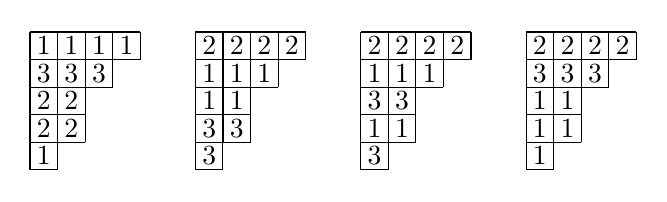
\begin{tikzpicture}[scale=0.35]
    % Tableau 1
    \begin{scope}[shift={(0,0)}]
        \node at (0.5, 0.5) {1}; \node at (1.5, 0.5) {1}; \node at (2.5, 0.5) {1}; \node at (3.5, 0.5) {1};
        \node at (0.5, -0.5) {3}; \node at (1.5, -0.5) {3}; \node at (2.5, -0.5) {3};
        \node at (0.5, -1.5) {2}; \node at (1.5, -1.5) {2};
        \node at (0.5, -2.5) {2}; \node at (1.5, -2.5) {2};
        \node at (0.5, -3.5) {1};
        \draw (0,0) grid (4,1); \draw (0,-1) grid (3,0); \draw (0,-2) grid (2,-1); \draw (0,-3) grid (2,-2); \draw (0,-4) grid (1,-3);
    \end{scope}
    
    % Tableau 2
    \begin{scope}[shift={(6,0)}]
        \node at (0.5, 0.5) {2}; \node at (1.5, 0.5) {2}; \node at (2.5, 0.5) {2}; \node at (3.5, 0.5) {2};
        \node at (0.5, -0.5) {1}; \node at (1.5, -0.5) {1}; \node at (2.5, -0.5) {1};
        \node at (0.5, -1.5) {1}; \node at (1.5, -1.5) {1};
        \node at (0.5, -2.5) {3}; \node at (1.5, -2.5) {3};
        \node at (0.5, -3.5) {3};
        \draw (0,0) grid (4,1); \draw (0,-1) grid (3,0); \draw (0,-2) grid (2,-1); \draw (0,-3) grid (2,-2); \draw (0,-4) grid (1,-3);
    \end{scope}
    
    % Tableau 3
    \begin{scope}[shift={(12,0)}]
        \node at (0.5, 0.5) {2}; \node at (1.5, 0.5) {2}; \node at (2.5, 0.5) {2}; \node at (3.5, 0.5) {2};
        \node at (0.5, -0.5) {1}; \node at (1.5, -0.5) {1}; \node at (2.5, -0.5) {1};
        \node at (0.5, -1.5) {3}; \node at (1.5, -1.5) {3};
        \node at (0.5, -2.5) {1}; \node at (1.5, -2.5) {1};
        \node at (0.5, -3.5) {3};
        \draw (0,0) grid (4,1); \draw (0,-1) grid (3,0); \draw (0,-2) grid (2,-1); \draw (0,-3) grid (2,-2); \draw (0,-4) grid (1,-3);
    \end{scope}

    % Tableau 4
    \begin{scope}[shift={(18,0)}]
        \node at (0.5, 0.5) {2}; \node at (1.5, 0.5) {2}; \node at (2.5, 0.5) {2}; \node at (3.5, 0.5) {2};
        \node at (0.5, -0.5) {3}; \node at (1.5, -0.5) {3}; \node at (2.5, -0.5) {3};
        \node at (0.5, -1.5) {1}; \node at (1.5, -1.5) {1};
        \node at (0.5, -2.5) {1}; \node at (1.5, -2.5) {1};
        \node at (0.5, -3.5) {1};
        \draw (0,0) grid (4,1); \draw (0,-1) grid (3,0); \draw (0,-2) grid (2,-1); \draw (0,-3) grid (2,-2); \draw (0,-4) grid (1,-3);
    \end{scope}
\end{tikzpicture}
\end{center}
Hence, $M_{(4,3,2,2,1),(5,4,3)}(p,m) = 4$.

\textbf{Note:} The matrix for $k = 3$ is upper triangular and has non-zero determinant.

\newpage

% --- Source PDF page 15 ---
\section{The matrix \texorpdfstring{$[M_{\lambda,\mu}(p,m)]$}{[M\_\{lambda,mu\}(p,m)]} is triangular}

\begin{ptcb}
\begin{Prop}
Let $\lambda, \mu \vdash k$ with $|\lambda| = |\mu|$. Then:
\begin{enumerate}[(i)]
    \item If $\lambda >_{\text{lex}} \mu$, then $M_{\lambda,\mu}(p,m) = 0$.
    \item $M_{\lambda,\lambda}(p,m) > 0$.
\end{enumerate}
\end{Prop}
\end{ptcb}

\begin{proof}
(i) and (ii) Since $p_\lambda = p_{\lambda_1} p_{\lambda_2} \dots p_{\lambda_{\ell(\lambda)}}$ and $M_{\lambda,\mu}(p,m)$ is the coefficient of $x_1^{\mu_1} x_2^{\mu_2} \dots x_{\ell(\mu)}^{\mu_{\ell(\mu)}}$, we expand:
\[
p_\lambda = (x_1^{\lambda_1} + x_2^{\lambda_1} + \dots)(x_1^{\lambda_2} + x_2^{\lambda_2} + \dots) \dots (x_1^{\lambda_{\ell(\lambda)}} + x_2^{\lambda_{\ell(\lambda)}} + \dots)
\]
A factor in this product is obtained by picking one term $x_{i_j}^{\lambda_j}$ from the $j$-th factor. Suppose we pick $x_{i_1}^{\lambda_1}, x_{i_2}^{\lambda_2}, \dots, x_{i_{\ell(\lambda)}}^{\lambda_{\ell(\lambda)}}$. If $i_1, i_2, \dots, i_{\ell(\lambda)}$ are all distinct, then the product of these variables is $x_1^{\mu_1} x_2^{\mu_2} \dots x_{\ell(\mu)}^{\mu_{\ell(\mu)}}$ only if $\lambda = \mu$. We can form this product in $m_1(\lambda)! m_2(\lambda)! \dots m_{\ell(\lambda)}(\lambda)!$ ways, where $m_i(\lambda)$ is the multiplicity of $i$ in $\lambda$. This number is strictly positive, hence $M_{\lambda,\lambda}(p,m) > 0$.

If $i_1, i_2, \dots, i_{\ell(\lambda)}$ are not all distinct, then some $\mu_i$'s are sums of $\lambda_j$'s. This implies that there is a first part in $\mu$ that is strictly greater than the corresponding part in $\lambda$, so $\mu >_{\text{lex}} \lambda$. Thus, if $\lambda >_{\text{lex}} \mu$, we have $M_{\lambda,\mu}(p,m) = 0$.
\end{proof}

\newpage

% --- Source PDF page 16 ---
\section{The power sum symmetric functions form a basis}

\begin{ptcb}
\begin{Prop}
The set $\{p_\lambda \mid \lambda \vdash k\}$ is a basis for $\Lambda^k$, called the \textcolor{red}{power sum symmetric basis}.
\end{Prop}
\end{ptcb}

\begin{proof}
Let $A$ be the $p(k) \times p(k)$ matrix with rows and columns indexed by partitions of $k$ ordered lexicographically, with entries $M_{\lambda,\mu}(p,m)$. Then $A$ is upper triangular with non-zero diagonal entries. Hence $A$ is invertible, so it is the change of basis matrix from the $p$ basis to the $m$ basis.
\end{proof}

\textbf{Example:} For $k = 4$, the change of basis matrix $A$ (with rows and columns ordered $(1^4), (2,1^2), (2^2), (3,1), (4)$) is:
\[
A = \begin{bmatrix}
24 & 12 & 6 & 4 & 1 \\
0 & 2 & 2 & 2 & 1 \\
0 & 0 & 2 & 0 & 1 \\
0 & 0 & 0 & 1 & 1 \\
0 & 0 & 0 & 0 & 1
\end{bmatrix}
\]

\begin{ptcb}
\textbf{Generating Function for Power Sum Symmetric Functions:}
\[
P(t) = \sum_{k=1}^\infty \frac{p_k}{k} t^k = \log \left( \prod_{i=1}^\infty \frac{1}{1 - x_i t} \right)
\]
\end{ptcb}

\begin{proof}
From calculus, $\log \left( \frac{1}{1 - x} \right) = \sum_{n=1}^\infty \frac{1}{n} x^n$. Therefore,
\[
P(t) = \sum_{k=1}^\infty \frac{p_k}{k} t^k = \sum_{k=1}^\infty \sum_{i=1}^\infty \frac{1}{k} (x_i t)^k = \sum_{i=1}^\infty \log \left( \frac{1}{1 - x_i t} \right) = \log \left( \prod_{i=1}^\infty \frac{1}{1 - x_i t} \right)
\]
\end{proof}

\chapter{Schur Symmetric Functions}

\section*{Lecture 3: Schur Symmetric Functions}
\begin{center}
\textbf{Rosa Orellana} \\
Dartmouth College \\
CIMPA-ECCO Summer School, August 5, 2026
\end{center}

\section{Definitions and Tableaux}

\begin{ptcb}
\begin{Def}
Let $\lambda$ be a partition. A \textbf{Young tableau} (or simply tableau) $T$ of shape $\lambda$ is a filling of the boxes of the Young diagram of $\lambda$ with positive integers.

The \textbf{weight} (or content) of $T$, denoted $x^T$, is defined by
\[
x^T = \prod_{i \in T} x_i = x_1^{c_1} x_2^{c_2} \cdots
\]
where $c_i$ is the number of times $i$ appears in $T$.
\end{Def}
\end{ptcb}

We define three special classes of tableaux of shape $\lambda$.  In each
case there is no condition relating entries in different rows:
\begin{itemize}
    \item $\text{StrictRow}(\lambda)$: The set of tableaux that are \textcolor{red}{strictly increasing} along each row.
    \item $\text{WeakRow}(\lambda)$: The set of tableaux that are \textcolor{red}{weakly increasing} along each row.
    \item $\text{ConstantRow}(\lambda)$: The set of tableaux that are \textcolor{red}{constant} along each row.
\end{itemize}

\begin{ptcb}
\begin{Prop}
The elementary, homogeneous, and power sum symmetric functions can be expressed as sums over tableaux:
\[
e_\lambda = \sum_{T \in \text{StrictRow}(\lambda)} x^T, \quad h_\lambda = \sum_{T \in \text{WeakRow}(\lambda)} x^T, \quad p_\lambda = \sum_{T \in \text{ConstantRow}(\lambda)} x^T
\]
\end{Prop}
\end{ptcb}

\newpage

\section{Schur Functions Definition}

\begin{ptcb}
\begin{Def}
A \textbf{semi-standard Young tableau (SSYT)} of shape $\lambda$ is a filling of the boxes of $\lambda$ with positive integers such that:
\begin{enumerate}
    \item Entries are \textcolor{red}{weakly increasing} across each row from left to right.
    \item Entries are \textcolor{red}{strictly increasing} down each column from top to bottom.
\end{enumerate}
We write $SST(\lambda)$ for the set of all semi-standard Young tableaux of shape $\lambda$, and $SST(\lambda, \mu)$ for the set of semi-standard Young tableaux of shape $\lambda$ with content $\mu$.
\end{Def}
\end{ptcb}

\begin{ptcb}
\begin{Def}
For any partition $\lambda$, the \textbf{Schur function} $s_\lambda$ is defined by
\[
s_\lambda = \sum_{T \in SST(\lambda)} x^T
\]
\end{Def}
\end{ptcb}

\begin{ptcb}
\begin{Ex}
Compute $s_{2,1}(x_1, x_2, x_3)$. The shape $\lambda = (2,1)$ has 3 boxes. The semi-standard Young tableaux filled with $\{1,2,3\}$ are:
\[
\ytableaushort{11,2}, \quad \ytableaushort{11,3}, \quad \ytableaushort{12,2}, \quad \ytableaushort{12,3}, \quad \ytableaushort{13,2}, \quad \ytableaushort{13,3}, \quad \ytableaushort{22,3}, \quad \ytableaushort{23,3}
\]
Evaluating their weights yields:
\[
s_{2,1}(x_1, x_2, x_3) = m_{2,1}(x_1, x_2, x_3) + 2 m_{1,1,1}(x_1, x_2, x_3)
\]
\end{Ex}
\end{ptcb}

\newpage

\section{Special Cases: \texorpdfstring{$s_{1^k}$}{s_{1^k}} and \texorpdfstring{$s_k$}{s_k}}

\begin{ptcb}
\begin{Prop}
For any positive integer $k$:
\begin{enumerate}
    \item $s_{1^k} = e_k$.
    \item $s_k = h_k$.
\end{enumerate}
\end{Prop}
\end{ptcb}

\begin{proof}
\begin{enumerate}
    \item The shape $(1^k)$ is a single column of $k$ boxes. A filling is semi-standard if and only if the entries strictly increase from top to bottom: $1 \le i_1 < i_2 < \dots < i_k$. Thus,
    \[
    s_{1^k} = \sum_{1 \le i_1 < i_2 < \dots < i_k} x_{i_1} x_{i_2} \cdots x_{i_k} = e_k
    \]
    \item The shape $(k)$ is a single row of $k$ boxes. A filling is semi-standard if and only if the entries weakly increase from left to right: $1 \le i_1 \le i_2 \le \dots \le i_k$. Thus,
    \[
    s_k = \sum_{1 \le i_1 \le i_2 \le \dots \le i_k} x_{i_1} x_{i_2} \cdots x_{i_k} = h_k
    \]
\end{enumerate}
\end{proof}

\newpage

\section{Symmetry of Schur Functions}

\begin{ptcb}
\begin{Th}
For any partition $\lambda$, the Schur function $s_\lambda$ is a symmetric function, i.e., $s_\lambda \in \Lambda$.
\end{Th}
\end{ptcb}

\begin{proof}[Outline of Proof via Bender-Knuth Involution]
To show that $s_\lambda$ is symmetric, it suffices to show that swapping adjacent variables $x_i$ and $x_{i+1}$ leaves $s_\lambda$ invariant. This is done by defining an involution $\phi_i$ on $SST(\lambda)$ that maps a tableau of weight $(\dots, \mu_i, \mu_{i+1}, \dots)$ to a tableau of weight $(\dots, \mu_{i+1}, \mu_i, \dots)$.

In any tableau $T \in SST(\lambda)$, call an entry $i$ or $i+1$ \emph{matched} if they appear in the same column (so $i$ is directly above $i+1$). All other entries $i$ and $i+1$ are \emph{free}. In each row, the free entries form a contiguous block of $i$'s followed by $(i+1)$'s. The involution $\phi_i$ replaces a block of $a$ $i$'s and $b$ $(i+1)$'s with $b$ $i$'s and $a$ $(i+1)$'s. This preserves semi-standardness and bijectively pairs tableaux with weight $x^T$ and $x^{\phi_i(T)}$, proving $|SST(\lambda, \mu)| = |SST(\lambda, \tilde{\mu})|$.
\end{proof}

\newpage

\section{The Kostka Numbers}

\begin{ptcb}
\begin{Def}
The \textbf{Kostka numbers} $K_{\lambda, \mu}$ are defined by
\[
s_\lambda = \sum_{\mu \vdash |\lambda|} K_{\lambda, \mu} m_\mu
\]
Equivalently, $K_{\lambda, \mu} = |SST(\lambda, \mu)|$ is the number of semi-standard Young tableaux of shape $\lambda$ and content $\mu$.
\end{Def}
\end{ptcb}

\begin{Ex}
For $k=3$, ordering partitions lexicographically as $(3), (2,1), (1,1,1)$, the Kostka matrix $K^{(3)} = (K_{\lambda, \mu})$ is:
\[
K^{(3)} = \begin{pmatrix}
1 & 1 & 1 \\
0 & 1 & 2 \\
0 & 0 & 1
\end{pmatrix}
\]
For $k=4$, ordering partitions as $(4), (3,1), (2,2), (2,1,1), (1,1,1,1)$, the Kostka matrix $K^{(4)}$ is:
\[
K^{(4)} = \begin{pmatrix}
1 & 1 & 1 & 1 & 1 \\
0 & 1 & 1 & 2 & 3 \\
0 & 0 & 1 & 1 & 2 \\
0 & 0 & 0 & 1 & 3 \\
0 & 0 & 0 & 0 & 1
\end{pmatrix}
\]
\end{Ex}

\newpage

\section{Schur Functions Form a Basis}

\begin{ptcb}
\begin{Th}
For any partitions $\lambda, \mu \vdash k$:
\begin{enumerate}
    \item $K_{\lambda, \mu} = 0$ if $\mu >_{\text{lex}} \lambda$.
    \item $K_{\lambda, \lambda} = 1$.
\end{enumerate}
Consequently, the set $\{s_\lambda \mid \lambda \vdash k\}$ forms a basis for the space of homogeneous symmetric functions of degree $k$, $\Lambda^k$.
\end{Th}
\end{ptcb}

\begin{proof}
If $\mu >_{\text{lex}} \lambda$, there is no semi-standard tableau of shape $\lambda$ and content $\mu$, because the entries $1, 2, \dots, i$ must all fit into the first $i$ rows, which is impossible if $\mu_1 + \dots + \mu_i > \lambda_1 + \dots + \lambda_i$. For $\mu = \lambda$, the unique SSYT of shape $\lambda$ and content $\lambda$ has row $i$ filled entirely with $i$, so $K_{\lambda,\lambda} = 1$. Thus the transition matrix $(K_{\lambda, \mu})$ is upper triangular with $1$s on the diagonal, so it is invertible.
\end{proof}

\newpage

\section{The Jacobi-Trudi Identity}

\begin{ptcb}
\begin{Th}[Jacobi-Trudi Identity]
Let $\lambda = (\lambda_1, \lambda_2, \dots, \lambda_k)$ be a partition. Then the Schur function $s_\lambda$ can be written as a determinant of complete homogeneous symmetric functions:
\[
s_\lambda = \det \left[ h_{\lambda_i + j - i} \right]_{1 \le i, j \le k}
\]
where by convention $h_0 = 1$ and $h_m = 0$ for $m < 0$.
\end{Th}
\end{ptcb}

In matrix form:
\[
s_\lambda = \begin{vmatrix}
h_{\lambda_1} & h_{\lambda_1 + 1} & h_{\lambda_1 + 2} & \cdots & h_{\lambda_1 + k - 1} \\
h_{\lambda_2 - 1} & h_{\lambda_2} & h_{\lambda_2 + 1} & \cdots & h_{\lambda_2 + k - 2} \\
h_{\lambda_3 - 2} & h_{\lambda_3 - 1} & h_{\lambda_3} & \cdots & h_{\lambda_3 + k - 3} \\
\vdots & \vdots & \vdots & \ddots & \vdots \\
h_{\lambda_k - k + 1} & h_{\lambda_k - k + 2} & h_{\lambda_k - k + 3} & \cdots & h_{\lambda_k}
\end{vmatrix}
\]

\newpage

\section{Jacobi-Trudi Determinant Examples}

\begin{ptcb}
\begin{Ex}
\begin{enumerate}
    \item For $\lambda = (2,1)$ with $k=2$:
    \[
    s_{2,1} = \begin{vmatrix} h_2 & h_3 \\ h_0 & h_1 \end{vmatrix} = h_2 h_1 - h_3 h_0 = h_{2,1} - h_3
    \]
    \item For $\lambda = (3,2,1)$ with $k=3$:
    \[
    s_{3,2,1} = \begin{vmatrix}
    h_3 & h_4 & h_5 \\
    h_1 & h_2 & h_3 \\
    h_{-1} & h_0 & h_1
    \end{vmatrix}
    = \begin{vmatrix}
    h_3 & h_4 & h_5 \\
    h_1 & h_2 & h_3 \\
    0 & 1 & h_1
    \end{vmatrix}
    \]
\end{enumerate}
\end{Ex}
\end{ptcb}

\newpage

\section{The Omega Involution}

\begin{ptcb}
\begin{Def}
The \textbf{omega map} $\omega: \Lambda \to \Lambda$ is the algebra homomorphism defined on the elementary generators by
\[
\omega(e_n) = h_n \quad \text{for all } n \ge 1
\]
\end{Def}
\end{ptcb}

\begin{ptcb}
\begin{Prop}[Properties of \texorpdfstring{$\omega$}{\omega}]
\begin{enumerate}
    \item $\omega$ is an involution: $\omega^2 = \text{id}$.
    \item $\omega(e_\lambda) = h_\lambda$ and $\omega(h_\lambda) = e_\lambda$.
    \item $\omega(s_\lambda) = s_{\lambda'}$, where $\lambda'$ is the conjugate partition of $\lambda$.
    \item $\omega(p_\lambda) = (-1)^{|\lambda| - \ell(\lambda)} p_\lambda$.
\end{enumerate}
\end{Prop}
\end{ptcb}

Applying $\omega$ to the Jacobi-Trudi identity yields the \textbf{Dual Jacobi-Trudi Identity}:
\[
s_{\lambda'} = \det \left[ e_{\lambda_i + j - i} \right]_{1 \le i, j \le k} \quad \Longleftrightarrow \quad s_\lambda = \det \left[ e_{\lambda'_i + j - i} \right]_{1 \le i, j \le \ell(\lambda')}
\]

\newpage

\section{Writing \texorpdfstring{$s_\lambda$}{s_{\lambda}} in the Elementary Basis}

\begin{ptcb}
\begin{Cor}
The Schur function $s_\lambda$ can be expanded in terms of the elementary symmetric functions using the dual Jacobi-Trudi formula:
\[
s_\lambda = \det \left[ e_{\lambda'_i + j - i} \right]_{1 \le i, j \le \ell(\lambda')}
\]
\end{Cor}
\end{ptcb}

\begin{ptcb}
\begin{Ex}
Compute $s_{3,2}$ in the elementary basis.
The conjugate of $\lambda = (3,2)$ is $\lambda' = (2,2,1)$, which has length $3$. Thus:
\[
s_{3,2} = \begin{vmatrix}
e_2 & e_3 & e_4 \\
e_1 & e_2 & e_3 \\
e_{-1} & e_0 & e_1
\end{vmatrix}
= \begin{vmatrix}
e_2 & e_3 & e_4 \\
e_1 & e_2 & e_3 \\
0 & 1 & e_1
\end{vmatrix}
\]
Expanding along the last row yields:
\[
s_{3,2} = -1 \cdot (e_2 e_3 - e_1 e_4) + e_1 (e_2^2 - e_1 e_3) = e_1 e_2^2 - e_1^2 e_3 - e_2 e_3 + e_1 e_4
\]
\end{Ex}
\end{ptcb}

\newpage

\section{The Forgotten Basis}

\begin{ptcb}
\begin{Def}
The \textbf{forgotten symmetric functions} $f_\lambda$ are defined by applying the $\omega$ involution to the monomial basis:
\[
f_\lambda = \omega(m_\lambda)
\]
\end{Def}
\end{ptcb}

\begin{ptcb}
\begin{Prop}
The set $\{f_\lambda \mid \lambda \vdash k\}$ forms a basis for $\Lambda^k$.
\end{Prop}
\end{ptcb}

\begin{Ex}
\begin{itemize}
    \item $f_{2,1} = \omega(m_{2,1}) = -2m_3 - m_{2,1}$
    \item $f_{1,1,1} = \omega(m_{1,1,1}) = m_{1,1,1} + m_{2,1} + m_3$
    \item $f_3 = \omega(m_3) = m_3$
    \item $f_{3,2} = \omega(m_{3,2}) = -m_{3,2} - 2m_5$
\end{itemize}
\end{Ex}

\newpage

\section{The Pieri Rules: Definitions}

\begin{ptcb}
\begin{Def}
Let $\mu \subseteq \lambda$ be partitions. The \textbf{skew diagram} $\lambda / \mu$ is the set of boxes belonging to $\lambda$ but not to $\mu$.
\end{Def}
\end{ptcb}

\begin{ptcb}
\begin{Def}
A \textbf{horizontal strip} is a skew diagram $\lambda / \mu$ that contains \textcolor{red}{at most one box in each column}.
\end{Def}
\end{ptcb}

\textit{Note}: Skew diagrams do not need to form a single connected piece.

\newpage

\section{The Pieri Rules for \texorpdfstring{$h_k$}{h_k}}

\begin{ptcb}
\begin{Th}[Pieri Rule for $h_k$]
For any partition $\mu$ and non-negative integer $k$:
\[
h_k s_\mu = \sum_{\lambda} s_\lambda
\]
where the sum is over all partitions $\lambda \supseteq \mu$ such that $\lambda / \mu$ is a \textbf{horizontal strip} of size $k$.
\end{Th}
\end{ptcb}

\begin{Ex}
Let $\mu = (2,2)$:
\begin{itemize}
    \item $h_1 s_{2,2} = s_{3,2} + s_{2,2,1}$
    \item $h_2 s_{2,2} = s_{4,2} + s_{3,2,1} + s_{2,2,2}$
    \item $h_3 s_{2,2} = s_{5,2} + s_{4,2,1} + s_{3,2,2}$
\end{itemize}
\end{Ex}

\newpage

\section{Expanding \texorpdfstring{$h_\mu$}{h_{\mu}} in the Schur Basis}

\begin{ptcb}
To write $h_\mu = h_{\mu_1} h_{\mu_2} \dots h_{\mu_\ell}$ in the Schur basis, we repeatedly apply the Pieri rule for horizontal strips, generating a tree of tableaux.
\end{ptcb}

\begin{Ex}
Expand $h_{3,2,1}$ in the Schur basis:
\begin{center}
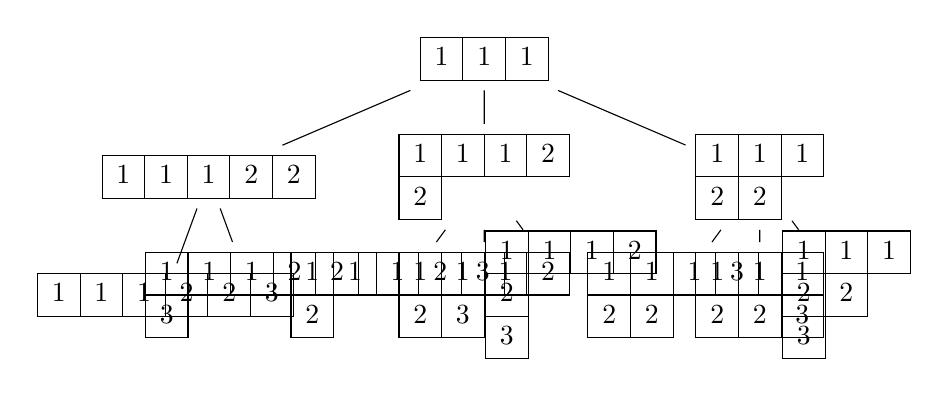
\begin{tikzpicture}[level distance=1.5cm,
  level 1/.style={sibling distance=3.5cm},
  level 2/.style={sibling distance=1.1cm}]
  \node {$\ytableaushort{111}$}
    child {node {$\ytableaushort{11122}$}
      child {node {$\ytableaushort{111223}$}}
      child {node {$\ytableaushort{11122,3}$}}
    }
    child {node {$\ytableaushort{1112,2}$}
      child {node {$\ytableaushort{11123,2}$}}
      child {node {$\ytableaushort{1112,23}$}}
      child {node {$\ytableaushort{1112,2,3}$}}
    }
    child {node {$\ytableaushort{111,22}$}
      child {node {$\ytableaushort{1113,22}$}}
      child {node {$\ytableaushort{111,223}$}}
      child {node {$\ytableaushort{111,22,3}$}}
    };
\end{tikzpicture}
\end{center}

Summing the shapes of the leaves gives:
\[
h_{3,2,1} = s_6 + 2 s_{5,1} + 2 s_{4,2} + s_{4,1,1} + s_{3,3} + s_{3,2,1}
\]
\end{Ex}

\newpage

\section{The Pieri Rules for \texorpdfstring{$e_k$}{e_k}}

\begin{ptcb}
\begin{Def}
A \textbf{vertical strip} is a skew diagram $\lambda / \mu$ that contains \textcolor{red}{at most one box in each row}.
\end{Def}
\end{ptcb}

\begin{ptcb}
\begin{Th}[Pieri Rule for $e_k$]
For any partition $\mu$ and non-negative integer $k$:
\[
e_k s_\mu = \sum_{\lambda} s_\lambda
\]
where the sum is over all partitions $\lambda \supseteq \mu$ such that $\lambda / \mu$ is a \textbf{vertical strip} of size $k$.
\end{Th}
\end{ptcb}

\begin{Ex}
Let $\mu = (2,2)$:
\begin{itemize}
    \item $e_2 s_{2,2} = s_{3,3} + s_{3,2,1} + s_{2,2,1,1}$
    \item $e_3 s_{2,2} = s_{3,3,1} + s_{3,2,1,1} + s_{2,2,1,1,1}$
\end{itemize}
\end{Ex}

\newpage

\section{Expanding \texorpdfstring{$e_\mu$}{e_{\mu}} in the Schur Basis}

\begin{ptcb}
To write $e_\mu = e_{\mu_1} e_{\mu_2} \dots e_{\mu_\ell}$ in the Schur basis, we repeatedly apply the Pieri rule for vertical strips.
\end{ptcb}

\begin{Ex}
Expand $e_{3,2,1}$ in the Schur basis:
\[
e_{3,2,1} = s_{3,2,1} + s_{2^3} + 2 s_{2^2,1^2} + s_{3,1^3} + 2 s_{2,1^4} + s_{1^6}
\]
\end{Ex}

\newpage

\section{The Murnaghan-Nakayama Rule}

\begin{ptcb}
\begin{Def}
A \textbf{border strip} (or ribbon) is a connected skew diagram $\lambda / \mu$ that contains no $2 \times 2$ square of boxes.

The \textbf{height} $h(B)$ of a border strip $B = \lambda / \mu$ is defined as
\[
h(B) = (\text{number of rows of } B) - 1
\]
\end{Def}
\end{ptcb}

\begin{ptcb}
\begin{Th}[Murnaghan-Nakayama Rule]
For any integer $k \ge 1$ and partition $\mu$:
\[
p_k s_\mu = \sum_{\lambda} (-1)^{h(\lambda / \mu)} s_\lambda
\]
where the sum is over all partitions $\lambda \supseteq \mu$ such that $\lambda / \mu$ is a \textbf{border strip} of size $k$.
\end{Th}
\end{ptcb}

\begin{Ex}
Compute $p_3 s_{6,3,3,2,1}$:
\[
p_3 s_{6,3,3,2,1} = s_{9,3,3,2,1} + s_{6,6,3,2,1} - s_{6,5,4,2,1} - s_{6,3,3,2,2,2} - s_{6,3,3,3,3} + s_{6,3,3,2,1,1,1,1}
\]
\end{Ex}

\chapter{The Chromatic Symmetric Function}

\section*{Lecture 4: The Chromatic Symmetric Function}
\begin{center}
\textbf{Rosa Orellana} \\
Dartmouth College \\
CIMPA-ECCO Summer School, August 6, 2026
\end{center}

\section{Introduction and Graphs}

\begin{ptcb}
\begin{Def}
A \textbf{graph} $G = (V, E)$ consists of a finite set of \textbf{vertices} (or nodes) $V = V(G)$ and a set of \textbf{edges} $E = E(G)$, where each edge is an unordered pair $\{u, v\}$ of distinct vertices. Vertices represent objects, and edges represent relationships between pairs of objects.
\end{Def}
\end{ptcb}

\begin{ptcb}
\begin{Def}
A \textbf{cycle} $C_k$ is a closed walk of $k$ distinct vertices $v_1, v_2, \dots, v_k$ such that $\{v_i, v_{i+1}\} \in E$ for all $1 \le i \le k-1$ and $\{v_k, v_1\} \in E$.

A graph $G$ is \textbf{connected} if there is a path between every pair of vertices. A \textbf{tree} is a connected graph with no cycles. Vertices of degree 1 in a tree are called \textbf{leaves}.
\end{Def}
\end{ptcb}

\newpage

\section{Colorings and the Chromatic Polynomial}

\begin{ptcb}
\begin{Def}
A \textbf{proper coloring} of a simple graph $G = (V, E)$ with $n$ colors is a map $\kappa: V \to \{1, 2, \dots, n\}$ such that if $\{u, v\} \in E$, then $\kappa(u) \neq \kappa(v)$.
\end{Def}
\end{ptcb}

\begin{ptcb}
\begin{Def}
The \textbf{chromatic polynomial} $\chi_G(n)$ counts the number of proper colorings of $G$ using at most $n$ colors.
\end{Def}
\end{ptcb}

\begin{Ex}
\begin{enumerate}
    \item For the triangle graph $C_3$:
    \[
    \chi_{C_3}(n) = n(n-1)(n-2)
    \]
    For $n=3$ colors, there are $\chi_{C_3}(3) = 3 \cdot 2 \cdot 1 = 6$ proper colorings.
    \item For any tree $T$ with $k$ vertices:
    \[
    \chi_T(n) = n(n-1)^{k-1}
    \]
\end{enumerate}
\end{Ex}

\textbf{Note:} The chromatic polynomial $\chi_G(n)$ cannot distinguish between non-isomorphic trees on the same number of vertices! For example, all trees on $k$ vertices have the exact same chromatic polynomial $\chi_T(n) = n(n-1)^{k-1}$.

\newpage

\section{The Chromatic Symmetric Function}

To capture more structural information about a graph, Richard Stanley (1995) introduced a symmetric function generalization of the chromatic polynomial.

\begin{ptcb}
\begin{Def}[Stanley, 1995]
Let $G = (V, E)$ be a simple graph with vertex set $V = \{v_1, v_2, \dots, v_n\}$. To each proper coloring $\kappa: V \to \mathbb{N}$, associate the monomial $x^\kappa = x_{\kappa(v_1)} x_{\kappa(v_2)} \dots x_{\kappa(v_n)}$.

The \textbf{chromatic symmetric function (CSF)} of $G$ is defined as
\[
\mathbf{X}_G(x_1, x_2, \dots) = \sum_{\kappa \text{ proper}} x_{\kappa(v_1)} x_{\kappa(v_2)} \dots x_{\kappa(v_n)}
\]
\end{Def}
\end{ptcb}

\begin{ptcb}
\begin{Prop}[Properties of the CSF]
\begin{enumerate}
    \item \textbf{Evaluation to Chromatic Polynomial:} 
    \[
    \mathbf{X}_G(\underbrace{1, 1, \dots, 1}_{n}, 0, 0, \dots) = \chi_G(n)
    \]
    \item \textbf{Disjoint Union:} If $G = H_1 \sqcup H_2$ is the disjoint union of graphs $H_1$ and $H_2$, then
    \[
    \mathbf{X}_G = \mathbf{X}_{H_1} \mathbf{X}_{H_2}
    \]
    \item \textbf{Symmetry:} $\mathbf{X}_G \in \Lambda$ is a homogeneous symmetric function of degree $|V(G)|$.
\end{enumerate}
\end{Prop}
\end{ptcb}

\newpage

\section{The CSF in the Power Basis}

For a subset of edges $S \subseteq E(G)$, let $\pi(S)$ be the integer partition whose parts are the vertex-sizes of the connected components of the spanning subgraph $(V(G), S)$.

\begin{ptcb}
\begin{Th}[Stanley, 1995]
For any graph $G = (V, E)$:
\[
\mathbf{X}_G = \sum_{S \subseteq E(G)} (-1)^{|S|} p_{\pi(S)}
\]
where $p_\lambda$ is the power sum symmetric function.
\end{Th}
\end{ptcb}

\begin{Ex}
Let $G$ be the 5-vertex graph formed by a triangle with two attached leaves (a "bull-like" graph). Summing over all $2^{|E|}$ edge subsets $S \subseteq E(G)$ according to component sizes yields:
\[
\mathbf{X}_G = p_{1^5} - 5 p_{2,1^3} + 2 p_{3,1^2} + 7 p_{2^2,1} - 4 p_{3,2} - 2 p_{4,1} + p_5
\]
\end{Ex}

\newpage

\section{Graph Invariants Recoverable from the CSF}

Expanding the CSF in the power basis $\mathbf{X}_G = \sum_{\lambda \vdash |V(G)|} a_\lambda p_\lambda$, many structural properties of $G$ can be extracted directly from the coefficients $a_\lambda$:

\begin{ptcb}
\begin{Prop}[Recoverable Invariants]
Let $G = (V, E)$ with $|V| = n$.
\begin{itemize}
    \item \textbf{Number of Vertices:} $|V| = |\lambda|$.
    \item \textbf{Number of Edges:} $|E| = -a_{(2, 1^{n-2})}$.
    \item \textbf{Number of Matchings of Size $k$:} Given by $(-1)^k a_{(2^k, 1^{n-2k})}$.
    \item \textbf{Number of Triangles:} [Orellana--Scott] The number of triangles in $G$ is
    \[
    \text{\# Triangles} = \binom{|E|}{2} - a_{(2, 2, 1^{n-4})} - a_{(3, 1^{n-3})}
    \]
    \item \textbf{Tree Recovery:} [Martin--Morin--Wagner] For trees, many parameters including the degree sequence can be recovered.
\end{itemize}
\end{Prop}
\end{ptcb}

\newpage

\section{The Star Basis of Symmetric Functions}

\begin{ptcb}
\begin{Def}
Let $St_k$ denote the star graph on $k$ vertices (one central vertex of degree $k-1$ connected to $k-1$ leaves). The chromatic symmetric function of $St_k$ is
\[
\mathfrak{st}_k := \mathbf{X}_{St_k} = \sum_{i=0}^{k-1} (-1)^i \binom{k-1}{i} p_{(i+1, 1^{k-1-i})}
\]
For any partition $\lambda = (\lambda_1, \lambda_2, \dots, \lambda_\ell)$, define
\[
\mathfrak{st}_\lambda := \mathfrak{st}_{\lambda_1} \mathfrak{st}_{\lambda_2} \dots \mathfrak{st}_{\lambda_\ell}
\]
\end{Def}
\end{ptcb}

\begin{Ex}
For $St_4$ (star graph on 4 vertices):
\[
\mathbf{X}_{St_4} = -p_4 + 3 p_{3,1} - 3 p_{2,1,1} + p_{1,1,1,1} = \mathfrak{st}_4
\]
\end{Ex}

\begin{ptcb}
\begin{Th}[Cho--van Willigenburg, 2016]
The set $\{\mathfrak{st}_\lambda \mid \lambda \vdash n\}$ forms a basis for the space of homogeneous symmetric functions of degree $n$, $\Lambda^n$.
\end{Th}
\end{ptcb}

\begin{Ex}[Trees in Star Basis]
\begin{itemize}
    \item Path $P_4$: $\mathbf{X}_{P_4} = \mathfrak{st}_4 - \mathfrak{st}_{3,1} + \mathfrak{st}_{2,2}$
    \item Star $St_4$: $\mathbf{X}_{St_4} = \mathfrak{st}_4$
\end{itemize}
\end{Ex}

\begin{Ex}[Unicyclic Graphs in Star Basis]
\begin{itemize}
    \item Triangle $C_3$: $\mathbf{X}_{C_3} = 2 \mathfrak{st}_3 - \mathfrak{st}_{2,1}$
    \item Dart graph: $\mathbf{X} = 2 \mathfrak{st}_5 - 2 \mathfrak{st}_{4,1} + \mathfrak{st}_{4,2}$
\end{itemize}
From the star basis expansion, the size of the cycle in a unicyclic graph can be recovered [Bingham, Johnston, Lawson, Orellana, Pan, and Sato (2025)].
\end{Ex}

\newpage

\section{Graph Isomorphism and the Tree Isomorphism Conjecture}

\begin{ptcb}
\begin{Def}
Two graphs $G$ and $H$ are \textbf{isomorphic} ($G \cong H$) if there exists a bijection $\phi: V(G) \to V(H)$ such that $\{u, v\} \in E(G)$ if and only if $\{\phi(u), \phi(v)\} \in E(H)$.
\end{Def}
\end{ptcb}

Isomorphic graphs always have the same chromatic symmetric function ($\mathbf{X}_G = \mathbf{X}_H$). However, Stanley (1995) showed that non-isomorphic graphs can share the same CSF.

\begin{ptcb}
\begin{Th}[Open Problem: Tree Isomorphism Conjecture]
If $T_1$ and $T_2$ are non-isomorphic trees, then $\mathbf{X}_{T_1} \neq \mathbf{X}_{T_2}$.
In other words, the chromatic symmetric function distinguishes trees up to isomorphism.
\end{Th}
\end{ptcb}

\textbf{Known Progress:}
\begin{itemize}
    \item Verified for all trees with $n \le 29$ vertices (Heil and Ji, 2019 — over 5.46 billion trees).
    \item Verified for caterpillar graphs (Loebl, Sereni, 2018).
    \item Verified for "proper" trees with diameter $\le 5$ (Aliste-Prieto, De Mier, Orellana, Zamora, 2022).
\end{itemize}

\newpage

\section{Proper Trees, Core, and Edge Operations}

\begin{ptcb}
\begin{Def}
Let $T$ be a tree.
\begin{itemize}
    \item A \textbf{leaf} is a vertex of degree 1. A \textbf{leaf edge} is an edge incident to a leaf.
    \item An \textbf{internal vertex} is a vertex of degree $> 1$.
    \item An \textbf{internal edge} is an edge whose endpoints are both internal vertices.
    \item A \textbf{proper tree} is a tree where every vertex is a leaf or adjacent to at least one leaf.
    \item The \textbf{core} of a tree is the weighted graph obtained by removing all leaves and labeling each remaining (internal) vertex with the number of leaves adjacent to it plus one.
\end{itemize}
\end{Def}
\end{ptcb}

\begin{ptcb}
\textbf{Edge Operations on Graphs:}
\begin{itemize}
    \item \textbf{Deletion ($G - e$):} Delete edge $e$ from $G$.
    \item \textbf{Dot-contraction ($(G/e) + v$):} Contract edge $e$ and add an isolated vertex $v$.
    \item \textbf{Leaf-contraction ($(G/e) + v + e'$):} Contract edge $e$, add isolated vertex $v$, and add a leaf edge $e'$ to the contracted vertex.
\end{itemize}
\end{ptcb}

\newpage

\section{Deletion-Near-Contraction (DNC)}

\begin{ptcb}
\begin{Th}[Aliste-Prieto, De Mier, Orellana, Zamora]
For any graph $G$ and any edge $e$:
\[
\mathbf{X}_G = \mathbf{X}_{G-e} - \mathbf{X}_{(G/e)+v} + \mathbf{X}_{(G/e)+v+e'}
\]
\end{Th}
\end{ptcb}

\begin{proof}[Notes on DNC]
\begin{itemize}
    \item DNC is applied only to \textbf{internal edges}.
    \item The only simple, connected graphs without internal edges are \textbf{star graphs}.
    \item Applying DNC recursively to internal edges computes the expansion of $\mathbf{X}_G$ in the \textbf{star basis} $\mathfrak{st}_\lambda$.
    \item \textbf{No Cancellations:} Each branch in the DNC recursion tree contributes directly to a non-zero term in the star expansion!
\end{itemize}
\end{proof}

\begin{Ex}[DNC Expansion of a Tree]
Applying DNC to a tree with internal edges yields:
\[
\mathbf{X}_T = \mathfrak{st}_{4,2,2} - \mathfrak{st}_{4,3,1} + \mathfrak{st}_{4,4} - \mathfrak{st}_{5,2,1} + \mathfrak{st}_{6,1,1} + \mathfrak{st}_{6,2} - 2 \mathfrak{st}_{7,1} + \mathfrak{st}_8
\]
\end{Ex}

\newpage

\section{Properties and Leading Partitions in the Star Basis}

Expanding $\mathbf{X}_G = \sum_{\lambda \vdash |V|} c_\lambda \mathfrak{st}_\lambda$ in the star basis:

\begin{ptcb}
\begin{Prop}
\begin{enumerate}
    \item $G$ is connected if and only if $c_{(n)} \neq 0$ (i.e. $\mathfrak{st}_{(n)}$ appears with non-zero coefficient).
    \item If $G = T$ is a tree, then $c_{(n)} = 1$.
    \item For hook partitions $(n-m, 1^m)$, the coefficient is:
    \[
    c_{n-m, 1^m} = (-1)^m \binom{I(T)}{m}
    \]
    where $I(T)$ is the number of internal edges in $T$. In particular, $|c_{n-m, 1}| = I(T)$.
\end{enumerate}
\end{Prop}
\end{ptcb}

\begin{ptcb}
\begin{Def}
The \textbf{leaf component partition} $\lambda_{LC(T)}$ of a tree $T$ is the integer partition whose parts are the vertex-orders of the connected components of $T \setminus I(T)$ (deleting all internal edges).

The \textbf{leading partition} $\lambda_{lead}$ of $\mathbf{X}_T$ is the smallest partition in lexicographic order occurring with non-zero coefficient in the star-expansion.
\end{Def}
\end{ptcb}

\begin{ptcb}
\begin{Th}[Gonzalez-Orellana-Tomba]
For any tree $T$, the leading partition equals the leaf component partition:
\[
\lambda_{lead} = \lambda_{LC}
\]
Furthermore, the leading coefficient $c_{\lambda_{lead}}$ is given by
\[
c_{\lambda_{lead}} = (-1)^k \prod_{u_i} (\deg(u_i) - 1)
\]
where the product is over all vertices $u_i$ of degree greater than 1 in the core of $T$ having label 1, and $k$ is the number of such vertices.
\end{Th}
\end{ptcb}

\begin{Cor}
For all \textbf{proper trees}, $c_{\lambda_{lead}} = 1$ (since proper trees have no core vertices with label 1).
\end{Cor}

\end{document}
